\documentclass{article}
\usepackage[T1]{fontenc}
\usepackage[utf8]{inputenc}

\usepackage{cmbright}
\usepackage[T1]{fontenc}

\usepackage{multicol}

\usepackage{amsmath}
\usepackage{amsfonts}
\usepackage{amssymb}
\usepackage{tikz}
\usepackage{graphicx}
\graphicspath{  {./images/} }
\setlength{\parindent}{0pt}
\usepackage{changepage}
\usepackage{verbatim}
\usepackage{physics}
\usepackage{derivative}
\usepackage{bm}
\usepackage[colorlinks=true, linkcolor=blue, urlcolor=blue, citecolor=blue, anchorcolor=blue]{hyperref}

\addtolength{\oddsidemargin}{-.25in}
\addtolength{\textwidth}{0.5in}

\makeatletter
\newcommand*\bigcdot{\mathpalette\bigcdot@{.5}}
\newcommand*\bigcdot@[2]{\mathbin{\vcenter{\hbox{\scalebox{#2}{$\m@th#1\bullet$}}}}}
\makeatother

\DeclareMathOperator{\di}{d\!}
\newcommand*\Eval[3]{\left.#1\right\rvert_{#2}^{#3}}

\newcommand{\uvec}[1]{\boldsymbol{\hat{\textbf{#1}}}}
\newcommand{\vr}[1]{\textbf{#1}}

\newcommand{\thus}[0]{\; \; \longrightarrow \; \;}

\newcommand{\lag}{\mathcal{L}}
\newcommand{\ham}{\mathcal{H}}

\title{Distance Estimation Simulations}
\author{Ryan Liu}
\date{Last updated: \today}

\begin{document}

\maketitle

\section{Notes}

As in Section (3.5), the distance estimation function operates on the principle of parameter estimation. However, several updates were made:
\begin{itemize}
    \item In addition to limiting the number of iterations, the \textit{tolerance} parameter is added such that the function automatically terminates when a distance estimation lands within a specified difference from the desired SNR. This prevents unnecessary iterations that offer minimal improvements in accuracy. 
    \item Spin and sky location parameters are added to reflect the new expectation SNR calculation function. 
    \item To accommodate precession spin and reduce waveform generation time, the \textit{IMRPhenomPv2} model is used as opposed to \textit{SEOBNR4}, which offers approximately a 40-fold improvement in runtime. 
\end{itemize}

\section{Results}

\begin{figure}[!htb]
    \center{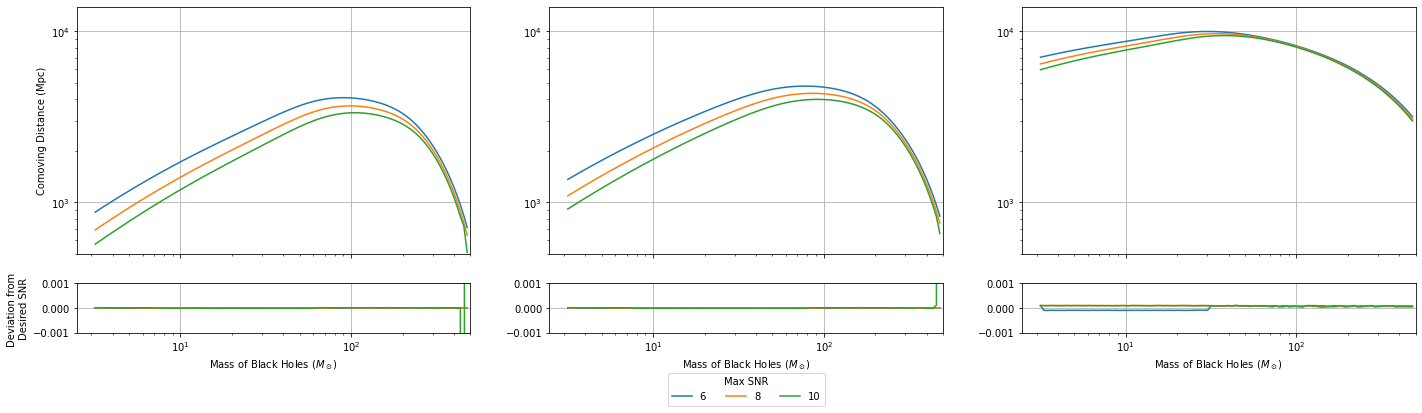
\includegraphics[width=\textwidth]{SNR26.png}}
    \caption{\label{fig:dist} (Top) Maximum comoving distance of detection for an equal-mass BBH at varying masses for (left to right) aLIGO, A+ aLIGO, and Cosmic Explorer design sensitivities. (Bottom) Deviation of parameter estimation from desired SNR}
\end{figure}

As seen in Figure \ref{fig:dist}, the component masses and frequency of orbit of BBH mergers have opposing effects on the maximum distance the merger can be observed. Due to the lower low-frequency cutoff for Cosmic Explorer (15 vs. 20 Hz), the mass-distance distribution peaks at a lower mass of around 30 $M_\odot$ rather than 90 $M_\odot$. \\

Because the SNR changes much more drastically for small changes in distance when the limiting factor is frequency rather than mass, it was necessary to use a significantly lower alpha rate when executing calculations for Cosmic Explorer design sensitivity. To speed up the overall parameter estimation function, it would be helpful to determine an analytic function to approximate the final distance, thereby reducing the number of iterations. \\

\begin{figure}[!htb]
    \center{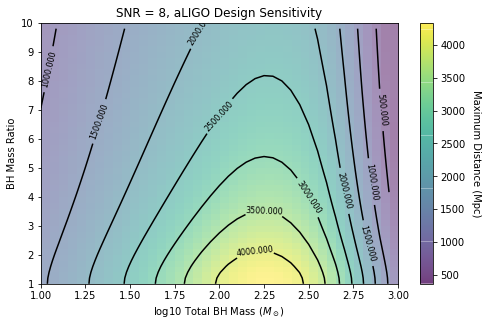
\includegraphics[width=2.5in]{SNR46.png}
    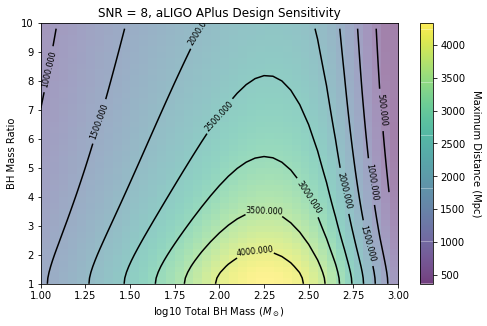
\includegraphics[width=2.5in]{SNR47.png}
    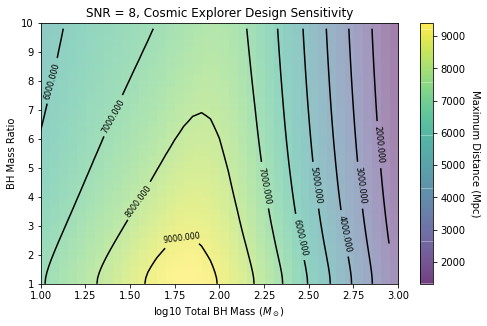
\includegraphics[width=2.5in]{SNR48.png}}
    \caption{\label{fig:dist} (Top) Maximum comoving distance of observation for zero-spin black holes of different total masses and mass ratios}
\end{figure}

\end{document}